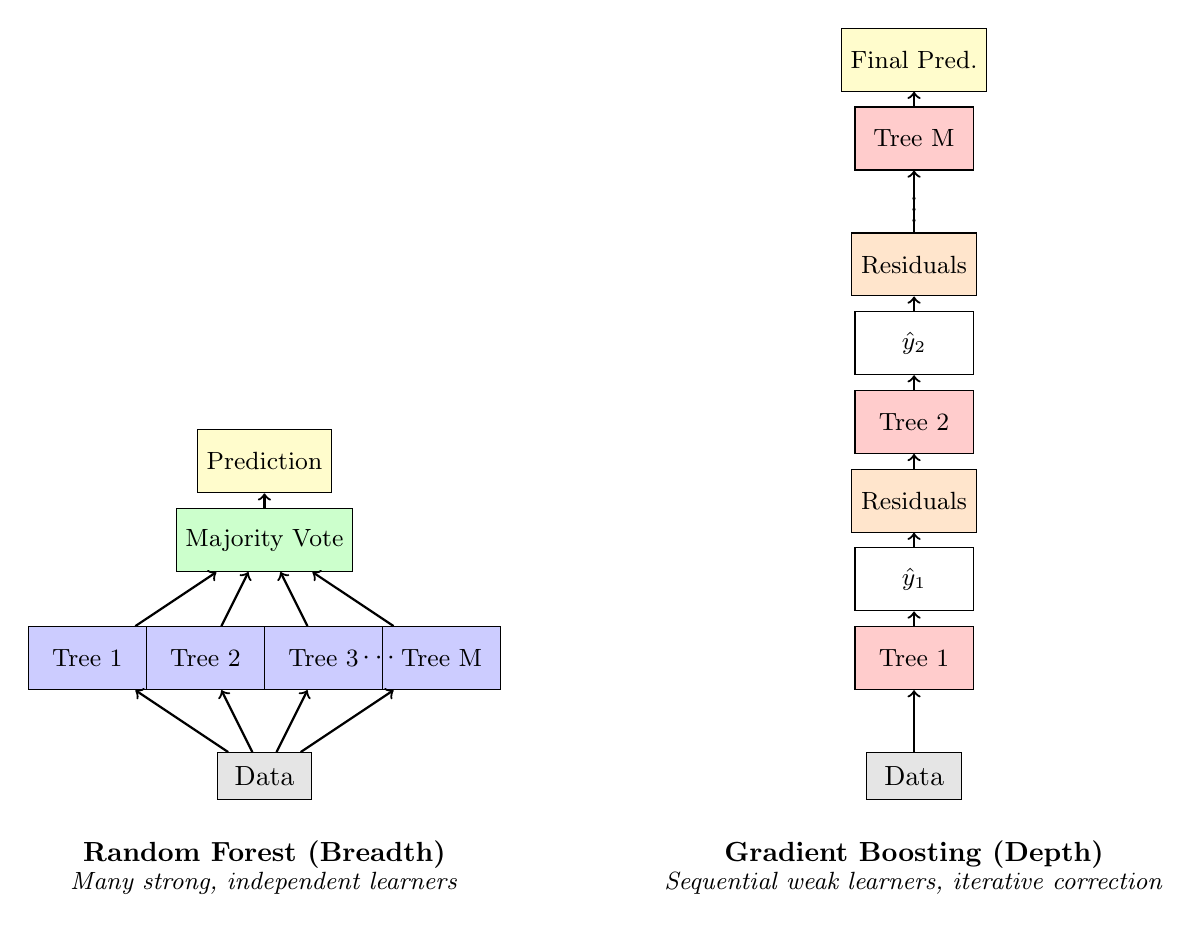
\begin{tikzpicture}[
  node distance=1cm,
  box/.style={rectangle,draw,minimum width=1.5cm,minimum height=0.8cm,font=\small},
  data/.style={rectangle,draw,minimum width=1.2cm,minimum height=0.6cm,fill=gray!20},
  decision/.style={rectangle,draw,minimum width=1cm,minimum height=0.6cm,fill=white},
  arrow/.style={->,thick}
]

% ===== RANDOM FOREST (Left) =====
\node[data] (data_rf) at (0.75,0) {Data};

% Trees trained in parallel
\node[box,fill=blue!20] (tree1) at (-1.5,1.5) {Tree 1};
\node[box,fill=blue!20] (tree2) at (0,1.5) {Tree 2};
\node[box,fill=blue!20] (tree3) at (1.5,1.5) {Tree 3};
\node[box,fill=blue!20] (tree_m) at (3,1.5) {Tree M};

% Parallel arrows
\draw[arrow] (data_rf) -- (tree1);
\draw[arrow] (data_rf) -- (tree2);
\draw[arrow] (data_rf) -- (tree3);
\draw[arrow] (data_rf) -- (tree_m);

% Add dots to indicate more trees
\node at (2.2,1.5) {$\cdots$};

% Aggregation
\node[box,fill=green!20] (agg) at (0.75,3) {Majority Vote};
\draw[arrow] (tree1) -- (agg);
\draw[arrow] (tree2) -- (agg);
\draw[arrow] (tree3) -- (agg);
\draw[arrow] (tree_m) -- (agg);

% Output
\node[box,fill=yellow!20] (out_rf) at (0.75,4) {Prediction};
\draw[arrow] (agg) -- (out_rf);

% Label
\node[font=\bfseries,anchor=north] at (0.75,-0.7) {Random Forest (Breadth)};
\node[font=\small,anchor=north] at (0.75,-1.1) {\textit{Many strong, independent learners}};

% ===== GRADIENT BOOSTING (Right) =====
\node[data] (data_gb) at (9,0) {Data};

% Sequential trees
\node[box,fill=red!20] (tree_1) at (9,1.5) {Tree 1};
\draw[arrow] (data_gb) -- (tree_1);

\node[box] (pred_1) at (9,2.5) {$\hat{y}_1$};
\draw[arrow] (tree_1) -- (pred_1);

\node[box,fill=orange!20] (residual_1) at (9,3.5) {Residuals};
\draw[arrow] (pred_1) -- (residual_1);

\node[box,fill=red!20] (tree_2) at (9,4.5) {Tree 2};
\draw[arrow] (residual_1) -- (tree_2);

\node[box] (pred_2) at (9,5.5) {$\hat{y}_2$};
\draw[arrow] (tree_2) -- (pred_2);

\node[box,fill=orange!20] (residual_2) at (9,6.5) {Residuals};
\draw[arrow] (pred_2) -- (residual_2);

% Add dots to indicate more iterations
\node[font=\large] at (9,7.3) {$\vdots$};

% Final output
\node[box,fill=red!20] (tree_m_gb) at (9,8.1) {Tree M};
\draw[arrow] (residual_2) -- (tree_m_gb);

\node[box,fill=yellow!20] (out_gb) at (9,9.1) {Final Pred.};
\draw[arrow] (tree_m_gb) -- (out_gb);

% Label
\node[font=\bfseries,anchor=north] at (9,-0.7) {Gradient Boosting (Depth)};
\node[font=\small,anchor=north] at (9,-1.1) {\textit{Sequential weak learners, iterative correction}};

\end{tikzpicture}
